\chapter{Cuestionario I}

\section{El flujo exhalatorio depende del ventilador o de las características de los pulmones del paciente?}

Cuando el proceso de exhalación finaliza los pulmones no se quedan completamente vacíos si no que queda un volumen mínimo residual para mantener el funcionamiento interno del mismo, es así que bajo este principio el ventilador adapta el nivel de exhalación según la respuesta pulmonar del paciente y el cual se puede configurar a partir de sus perillas en su sección de control.

\begin{figure}[h]
	\centering
	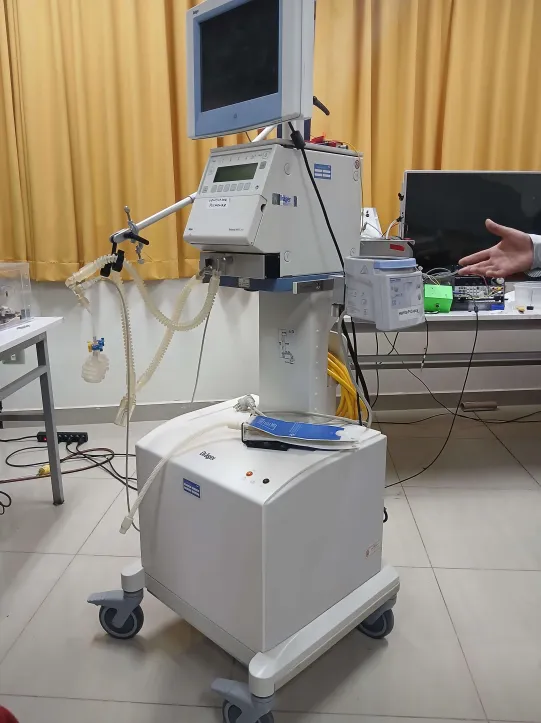
\includegraphics[width=0.7\linewidth]{media/vent-pulmonar}
	\caption{Ventilador pulmonar}
	\label{fig:vent-pulmonar}
\end{figure}

Y las cuales se encuentran en la parte superior del mismo, como se observa en la figura \ref{fig:vent-pulmonar}